% !TEX encoding = UTF-8
% !TEX TS-program = pdflatex
% !TEX root = ../tesi.tex
% !TEX spellcheck = it-IT

%**************************************************************
\chapter{Analisi dei requisiti}
\label{cap:analisi-requisiti}
%**************************************************************

\intro{Breve introduzione al capitolo}\\

\section{Casi d'uso}

Per lo studio dei casi di utilizzo del prodotto sono stati creati dei diagrammi.
I diagrammi dei casi d'uso (in inglese \emph{Use Case Diagram}) sono diagrammi di tipo \gls{uml} dedicati alla descrizione delle funzioni o servizi offerti da un sistema, così come sono percepiti e utilizzati dagli attori che interagiscono col sistema stesso.

%\begin{figure}[!h] 
%    \centering 
%    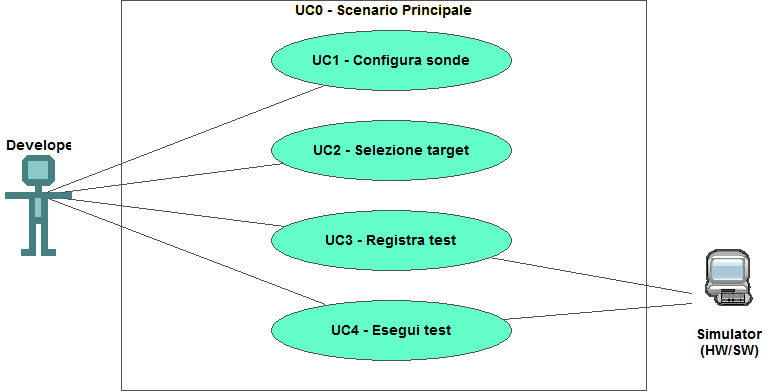
\includegraphics[width=0.9\columnwidth]{usecase/scenario-principale} 
%    \caption{Use Case - UC0: Scenario principale}
%\end{figure}

%\begin{usecase}{0}{Scenario principale}
%\usecaseactors{Sviluppatore applicativi}
%\usecasepre{Lo sviluppatore è entrato nel plug-in di simulazione all'interno dell'IDE}
%\usecasedesc{La finestra di simulazione mette a disposizione i comandi per configurare, registrare o eseguire un test}
%\usecasepost{Il sistema è pronto per permettere una nuova interazione}
%\label{uc:scenario-principale}
%\end{usecase}

\begin{figure}[!ht] 
    \centering 
    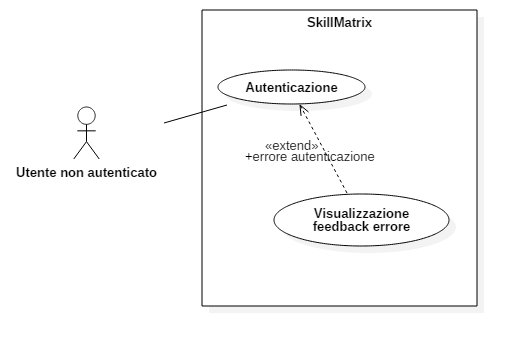
\includegraphics[width=0.9\columnwidth]{usecase/Autenticazione} 
    \caption{Use Case - Login}
\end{figure}

\begin{usecase}{1}{Autenticazione}
\usecaseactors{Utente non autenticato}
\usecasepre{l'utente non ha effettuato il login in SkillMatrix e deve possedere credenziali valide}
\usecasedesc{l'utente fornisce dei dati validi di accesso nella pagina di Login e viene reindirizzato alla pagina di gestione del profilo}
\usecasepost{le credenziali di accesso sono state verificate e l'utente è stato reindirizzato alla DASHBOARD}
\label{uc:autenticazione}
\end{usecase}

\begin{usecase}{2}{Visualizzazione feedback errore}
\usecaseactors{Utente non autenticato}
\usecasepre{l'utente non ha effettuato il login a SkillMatrix}
\usecasedesc{l'utente visualizza un messaggio d'errore nel caso in cui avvenga una delle seguenti situazioni:
\begin{itemize}
	\item le credenziali sono errate;
	\item la comunicazione con il server è fallita.
\end{itemize}}
\usecasepost{viene visualizzato un messaggio d'errore e il contatore che esprime la quantità di volte che l'errore si è manifestato, per poi far ritornare l'utente alla schermata di login}
\label{uc:errore_login}
\end{usecase}

\begin{figure}[!h] 
    \centering 
    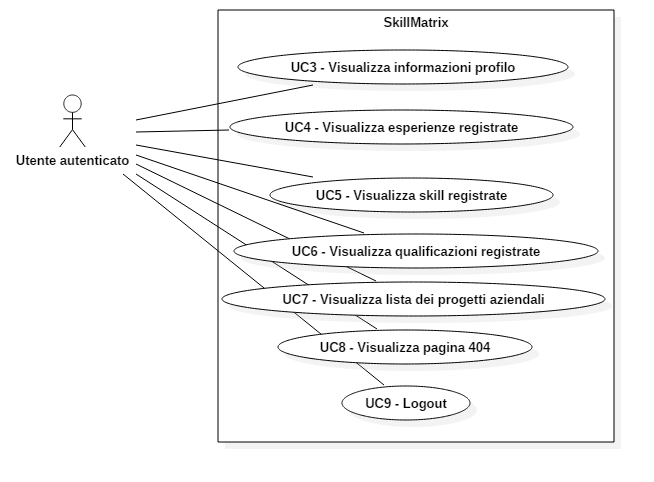
\includegraphics[width=0.9\columnwidth]{usecase/Dashboard} 
    \caption{Use Case - Dashboard}
\end{figure}

\begin{usecase}{3}{Visualizza informazioni profilo}
\usecaseactors{Utente autenticato}
\usecasepre{l'utente deve aver eseguito con successo il login al sistema}
\usecasedesc{l'utente seleziona il menù di visualizzazione delle informazioni del proprio profilo}
\usecasepost{l'utente viene reindirizzato alla pagina di presentazione delle proprie informazioni}
\label{uc:profilo}
\end{usecase}

\begin{usecase}{4}{Visualizza esperienze registrate}
\usecaseactors{Utente autenticato}
\usecasepre{l'utente deve aver eseguito con successo il login al sistema}
\usecasedesc{l'utente seleziona il menù di visualizzazione delle esperienze registrate nel sistema}
\usecasepost{l'utente viene reindirizzato alla pagina di presentazione delle proprie esperienze professionali registrate}
\label{uc:esperienze}
\end{usecase}

\begin{usecase}{5}{Visualizza skill registrate}
\usecaseactors{Utente autenticato}
\usecasepre{l'utente deve aver eseguito con successo il login al sistema}
\usecasedesc{l'utente seleziona il menù di visualizzazione delle skill registrate nel sistema}
\usecasepost{l'utente viene reindirizzato alla pagina di presentazione delle proprie skill registrate}
\label{uc:skill}
\end{usecase}

\begin{usecase}{6}{Visualizza qualificazioni registrate}
\usecaseactors{Utente autenticato}
\usecasepre{l'utente deve aver eseguito con successo il login al sistema}
\usecasedesc{l'utente seleziona il menù di visualizzazione delle qualificazioni registrate nel sistema}
\usecasepost{l'utente viene reindirizzato alla pagina di presentazione delle proprie qualificazioni registrate}
\label{uc:qualificazioni}
\end{usecase}

\begin{usecase}{7}{Visualizza lista dei progetti aziendali}
\usecaseactors{Utente autenticato}
\usecasepre{l'utente deve aver eseguito con successo il login al sistema}
\usecasedesc{l'utente seleziona il menù di visualizzazione dei progetti aziendali}
\usecasepost{l'utente viene reindirizzato alla pagina di visualizzazione della lista di progetti aziendali}
\label{uc:lista_progetti}
\end{usecase}

\begin{usecase}{8}{Visualizza pagina 404}
\usecaseactors{Utente autenticato}
\usecasepre{l'utente deve aver effettuato il login presso SkillMatrix ed avere una sessione attiva}
\usecasedesc{se l'utente, all'interno del dominio, effettua la ricerca di una risorsa non presente, il sistema informa l'utente di questa mancanza e fornisce istruzioni per la segnalazione}
\usecasepost{l'utente visualizza la pagina di segnalazione di risorsa non presente e decide se segnalare la mancanza o tornare alla DASHBOARD}
\label{uc:lista_progetti}
\end{usecase}

\begin{usecase}{9}{Logout}
\usecaseactors{Utente autenticato}
\usecasepre{l'utente deve aver effettuato il login presso SkillMatrix ed avere una sessione attiva}
\usecasedesc{l'utente seleziona il pulsante di logout presente nella dashboard}
\usecasepost{l'utente viene reindirizzato alla pagina di login e la sua sessiona viene cancellata}
\label{uc:logout}
\end{usecase}

\section{Tracciamento dei requisiti}

Da un'attenta analisi dei requisiti e degli use case effettuata sul progetto è stata stilata la tabella che traccia i requisiti in rapporto agli use case.\\
Sono stati individuati diversi tipi di requisiti e si è quindi fatto utilizzo di un codice identificativo per distinguerli.\\
Il codice dei requisiti è così strutturato R(F/Q/V)(N/D/O) dove:
\begin{enumerate}
	  \item[R =] requisito
    \item[F =] funzionale
    \item[Q =] qualitativo
    \item[V =] di vincolo
    \item[N =] obbligatorio (necessario)
    \item[D =] desiderabile
    \item[O =] opzionale
\end{enumerate}
Nelle tabelle \ref{tab:requisiti-funzionali}, \ref{tab:requisiti-qualitativi} e \ref{tab:requisiti-vincolo} sono riassunti i requisiti e il loro tracciamento con gli use case delineati in fase di analisi.

\newpage

\begin{table}%
\caption{Tabella del tracciamento dei requisti funzionali}
\label{tab:requisiti-funzionali}
\begin{tabularx}{\textwidth}{lXl}
\hline\hline
\textbf{Requisito} & \textbf{Descrizione} & \textbf{Use Case}\\
\hline
RFN-1 & L'applicazione deve reagire ad un'errata autenticazione tramite reindirizzamento all'interfaccia di login & UC2 \\
\hline
RFN-2 & L'applicazione deve reagire alla scadenza di una sessione tramite reindirizzamento all'interfaccia di login & UC2 \\
\hline
RFN-3 & L'applicazione non deve permettere l'accesso anonimo al sistema, tranne che per l'interfaccia di login & UC1 \\
\hline
RFN-4 & All'avvio, l'applicazione deve controllare se esiste una sessione attiva & - \\
\hline
RFN-5 & In caso di sessione attiva, l'utente deve essere reindirizzato alla Dashboard se la sessione è valida & - \\
\hline
RFN-6 & In caso di sessione non attiva o non valida, l'utente deve essere riportato alla schermata di login & UC2 \\
\hline
RFN-7 & L'applicazione deve poter consentire ad un utente registrato di effettuare l'autenticazione & UC1 \\
\hline
RFN-8 & L'utente autenticato deve poter visionare i propri dati dopo il login nel sistema & UC3 \\
\hline
RFN-9 & L'utente autenticato deve poter effettuare il logout dal sistema & UC9 \\
\hline
RFN-10 & L'utente deve poter visualizzare i propri titoli di studio e/o abilitazioni professionali una volta effettuato il login & UC6 \\
\hline
RFN-11 & L'utente deve poter inserire un nuovo titolo di studio o un'abilitazione professionale nel sistema & UCN \\
%%%%%%%%%%%%%%%%%%%%%%%%%%%%%%%%%%%%%%%%%%%%%%%%%%%%%%%%%%%%%%%%%%%%%%%%%%%%%%%%%%%%%%%%%%%%%%%%%%%
\hline
RFN-12 & L'utente deve poter visualizzare le proprie skill una volta effettuato il login & UC5 \\
\hline
RFN-12.1 & L'utente deve poter filtrare le skill visualizzate per livello di competenza & UCN \\
%%%%%%%%%%%%%%%%%%%%%%%%%%%%%%%%%%%%%%%%%%%%%%%%%%%%%%%%%%%%%%%%%%%%%%%%%%%%%%%%%%%%%%%%%%%%%%%%%%%
\hline
RFN-12.2 & L'utente deve poter inserire una nuova skill nel sistema & UCN \\
%%%%%%%%%%%%%%%%%%%%%%%%%%%%%%%%%%%%%%%%%%%%%%%%%%%%%%%%%%%%%%%%%%%%%%%%%%%%%%%%%%%%%%%%%%%%%%%%%%%
\hline
RFN-13 & L'utente deve poter visualizzare i progetti ad esso associati una volta effettuato il login & UC7 \\
\hline
RFN-13.1 & L'utente deve poter visualizzare quale progetto necessita di registrazione nel sistema & UCN \\
%%%%%%%%%%%%%%%%%%%%%%%%%%%%%%%%%%%%%%%%%%%%%%%%%%%%%%%%%%%%%%%%%%%%%%%%%%%%%%%%%%%%%%%%%%%%%%%%%%%
\hline
RFN-14 & L'utente deve poter visualizzare le informazioni dettagliate di un singolo progetto & UCN \\
%%%%%%%%%%%%%%%%%%%%%%%%%%%%%%%%%%%%%%%%%%%%%%%%%%%%%%%%%%%%%%%%%%%%%%%%%%%%%%%%%%%%%%%%%%%%%%%%%%%
\hline
RFN-15 & L'utente deve poter visualizzare le proprie esperienze professionali una volta effettuato il login al sistema & UC4 \\
\hline
RFN-16 & L'utente deve poter inserire una nuova esperienza professionale nel sistema & UCN \\
%%%%%%%%%%%%%%%%%%%%%%%%%%%%%%%%%%%%%%%%%%%%%%%%%%%%%%%%%%%%%%%%%%%%%%%%%%%%%%%%%%%%%%%%%%%%%%%%%%%
\hline
RFD-1 & Il sistema deve implementare una struttura gerarchica & UCN \\
%%%%%%%%%%%%%%%%%%%%%%%%%%%%%%%%%%%%%%%%%%%%%%%%%%%%%%%%%%%%%%%%%%%%%%%%%%%%%%%%%%%%%%%%%%%%%%%%%%%
\hline
RFD-1.1 & L'interfaccia mostrata in base al tipo di ogni utente deve essere adattata al tipo dello stesso & UCN \\
%%%%%%%%%%%%%%%%%%%%%%%%%%%%%%%%%%%%%%%%%%%%%%%%%%%%%%%%%%%%%%%%%%%%%%%%%%%%%%%%%%%%%%%%%%%%%%%%%%%
\hline
RFD-1.1.1 & L'amministratore di un progetto deve poter vedere le persone assegnate a quel progetto & UCN \\
%%%%%%%%%%%%%%%%%%%%%%%%%%%%%%%%%%%%%%%%%%%%%%%%%%%%%%%%%%%%%%%%%%%%%%%%%%%%%%%%%%%%%%%%%%%%%%%%%%%
\hline
RFD-2 & L'utente deve ricevere un feedback nell'interfaccia ogni volta che avvenga un errore di comunicazione col server & UCN \\
%%%%%%%%%%%%%%%%%%%%%%%%%%%%%%%%%%%%%%%%%%%%%%%%%%%%%%%%%%%%%%%%%%%%%%%%%%%%%%%%%%%%%%%%%%%%%%%%%%%
\hline
RFO-1 & Per tutti i dati presentati tramite lista va implementato l'infinite scroll & UCN \\
%%%%%%%%%%%%%%%%%%%%%%%%%%%%%%%%%%%%%%%%%%%%%%%%%%%%%%%%%%%%%%%%%%%%%%%%%%%%%%%%%%%%%%%%%%%%%%%%%%%
\hline
RFO-2 & L'utente deve poter visualizzare la quantità di progetti che richiedono registrazione tramite notifica nella dashboard & UCN \\
%%%%%%%%%%%%%%%%%%%%%%%%%%%%%%%%%%%%%%%%%%%%%%%%%%%%%%%%%%%%%%%%%%%%%%%%%%%%%%%%%%%%%%%%%%%%%%%%%%%
\hline
\end{tabularx}
\end{table}%

\begin{table}%
\caption{Tabella del tracciamento dei requisiti qualitativi}
\label{tab:requisiti-qualitativi}
\begin{tabularx}{\textwidth}{lXl}
\hline\hline
\textbf{Requisito} & \textbf{Descrizione} & \textbf{Use Case}\\
\hline
RQD-1 & Il codice deve seguire le linee stilistiche aziendali & - \\
\hline
RQD-2 & Deve venire prodotta la documentazione tecnica di dettaglio & - \\
\hline
RQD-3 & La grafica dell'interfaccia deve essere conforme agli standard aziendali & - \\
\hline
RQD-4 & L'utente deve visualizzare una pagina di supporto se naviga verso una pagina non presente & UC8 \\
\hline
\end{tabularx}
\end{table}%

\begin{table}%
\caption{Tabella del tracciamento dei requisiti di vincolo}
\label{tab:requisiti-vincolo}
\begin{tabularx}{\textwidth}{lXl}
\hline\hline
\textbf{Requisito} & \textbf{Descrizione} & \textbf{Use Case}\\
\hline
RVN-1 & Il framework di sviluppo per l'applicazione \gls{front-end} dev'essere AngularJS & Piano di Progetto \\
\hline
RVN-2 & La libreria \gls{css} da utilizzare dev'essere Bootstrap & Piano di Progetto \\
\hline
RVN-3 & Il framework di testing da utilizzare deve essere Jasmine & Piano di Progetto \\
\hline
RVN-4 & L'approccio di sviluppo deve essere Test Driven & Piano di Progetto \\
\hline
RVN-5 & Devono essere realizzate una o più componenti che simulino il \gls{back-end} in assenza di un server funzionante & - \\
\hline
RVN-6 & Le API definite devono rispettare il paradigma REST/HATEOAS & Piano di Progetto \\
\hline
RVN-6.1 & L'interfaccia deve poter manipolare correttamente gli header HTTP & - \\
\hline
RVN-7 & L'assegnamento dei ticket deve essere eseguito tramite il sistema kanban (JIRA) & - \\
\hline
RVN-8 & Il repository da utilizzare deve essere la configurazione aziendale di Atlassian STASH & - \\
\hline
RVN-9 & Lo schema dei dati associati ad un utente deve essere preso da schema.org & - \\
\hline
RVO-1 & I dati tabellari devono essere richiesti al server in maniera paginata & - \\
\hline
\end{tabularx}
\end{table}%

%****************************************************************

%\section{Mockup}
%Per rendere più chiaro sia visivamente che concettualmente il progetto da realizzare, all'inizio dell'analisi mi è stato fornito un file contenente la grafica e delle pagine di esempio dell'applicativo di SkillMatrix.\\
%Questo \emph{mockup} mi è servito come linea guida nello sviluppo grafico e del contenuto delle varie pagine dell'applicazione.